\subsubsection{Cenário otimista}

A Figura \ref{fig:cenario-otimista} apresenta as receitas e custos acumulados no cenário otimista considerando o projeto como um \gls{saas}. Nesse contexto, para o cálculo do acúmulo de receitas, estabeleceu-se um aumento mensal acentuado de 30 clientes para o plano básico e 25 para o profissional.

Os custos consideram somente os gastos com mão de obra, infraestrutura e mensalidades ou licenças das ferramentas utilizadas no desenvolvimento e manutenção da aplicação.

No cenário otimista, o ponto de equilíbrio é atingido no terceiro mês e, ao fim dos doze meses de análise, há um lucro de R\$ 253 mil.

\begin{figure}[h]
	\centering
	\caption{Cenário otimista}
	\fbox{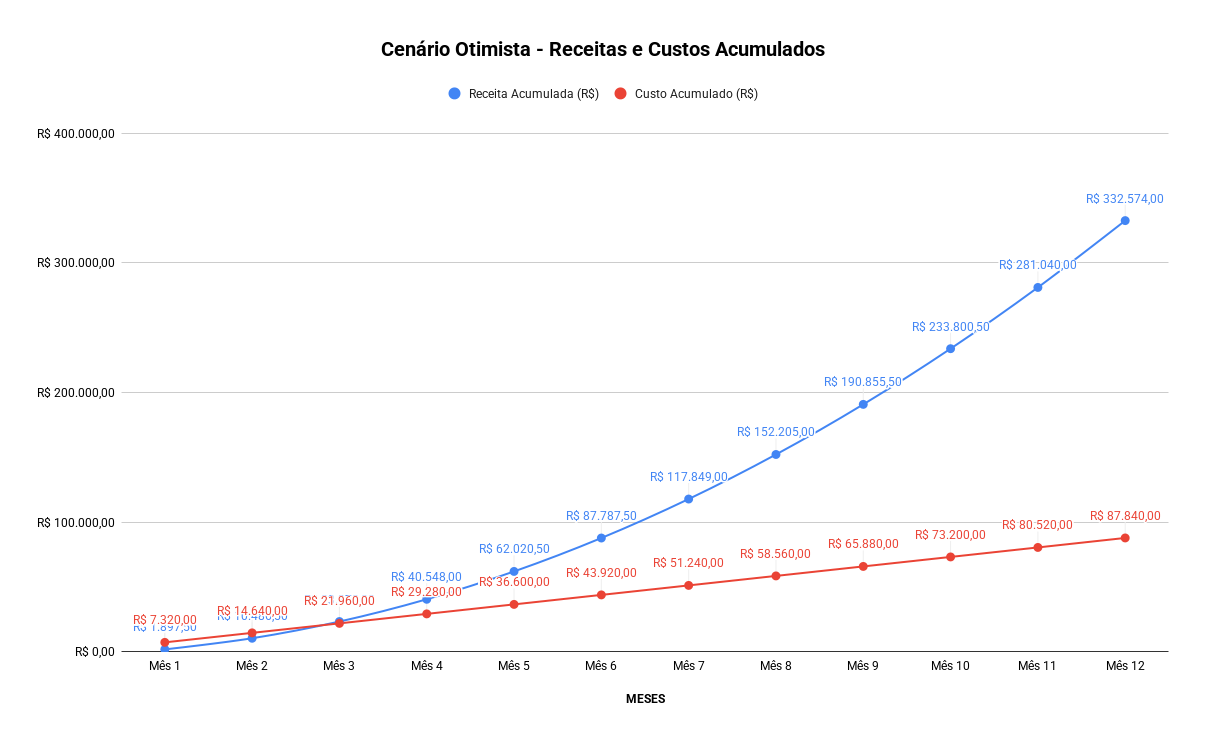
\includegraphics[width=0.9\textwidth]{cap05-viabilidade/imagens/cenario-otimista.png}}
	\label{fig:cenario-otimista}
	\fonte{Produzido pelos autores}
\end{figure}